\section{Useful tricks with {\twodx}}

In the present chapter we present you some tricks which might be useful in your daily usage of {\twodx}.

\subsection{Masking the Crystal}
\index{Masking}

In real world applications the crystal almost never fills the entire image as shown in \autoref{fig:mlk01_t}.

\begin{figure}[H]
	\centering
	\includegraphics[width=.85\textwidth]{mlk01.pdf}
	\caption{Non perfect crystal}
	\label{fig:mlk01_t}
\end{figure}

Therefore it does not make sense to use regions where the crystal is not regular or where we don't have any crystalline structure. {\twodx}\texttt{\_image} offers a tool with which you can manually mask an image. The following walkthrough explains how you can mask an your crystal.



\begin{enumerate}
	\item There are multiple ways how you can masked your image. The easiest way is to open the original image from the result panel of the initialization script and masked the image there. For many applications this does not work, as the crystal is not visible by eye. Thus we advise to masked in the file \textit{XCF Map for Manual Merging} which can be found in the result panel of \textit{Unbend II}. This file shows you the cross-correlation profile generated during unbending the crystal. The hight of the peak directly corresponds to the local quality of the crystal. In regions with no crystalline structures we will not find any peaks. \autoref{fig:mask_t_1} shows you the mentioned profile. As usual the file is opened in the fullscreen mode by a simple double click.
	
	\begin{figure}[H]
		\centering
		
\includegraphics[width=.85\textwidth]{mask_1.pdf}
		\caption{XCF Map for Manual Masking}
		\label{fig:mask_t_1}
	\end{figure}
	
	\item In order to be able to mask the image you have to activate the \textit{Polygon Selection Mode} by right-clicking in the image and selecting "Polygon Selection > Polygon Selection Masking" as shown in \autoref{fig:mask_t_2}.

	\begin{figure}[H]
		\centering
		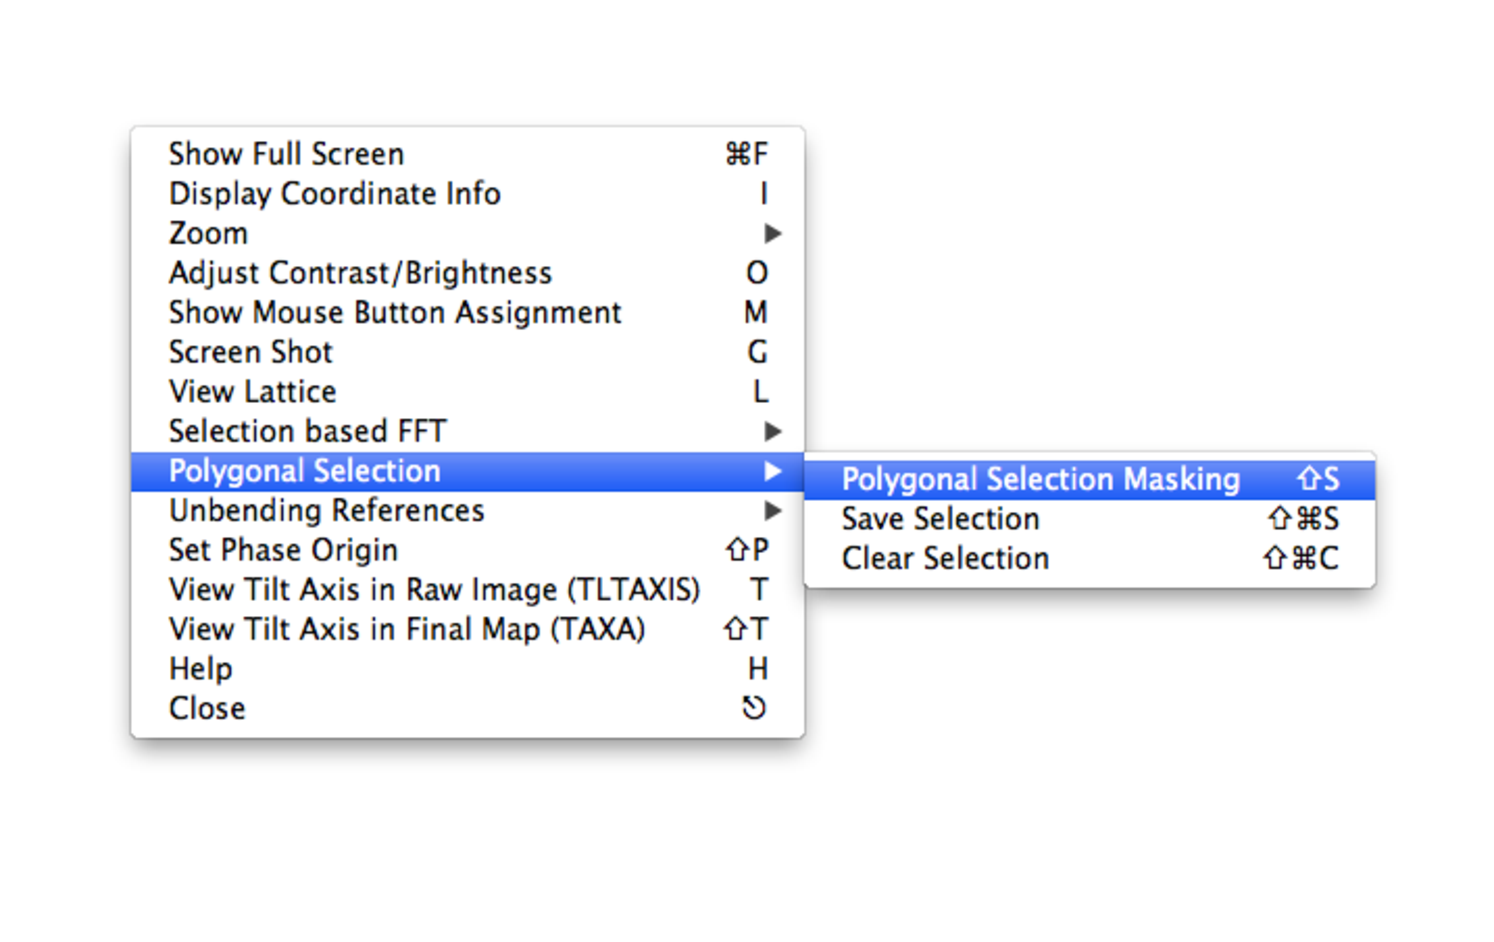
\includegraphics[width=.85\textwidth]{mask_2.pdf}
		\caption{Activate the Polygonal Mode}
		\label{fig:mask_t_2}
	\end{figure}
	
	\item Now you can mask your crystal by defining the borders with a bunch of left mouse clicks. A double-click will automatically close the selected polygon. Note that you can delete the current selection by selecting "Polygon Selection > Clear Selection" from the menu appearing when right-clicking on the image. Your masked image should be somehow similar to \autoref{fig:mask_t_3}.
	
	\begin{figure}[H]
		\centering
		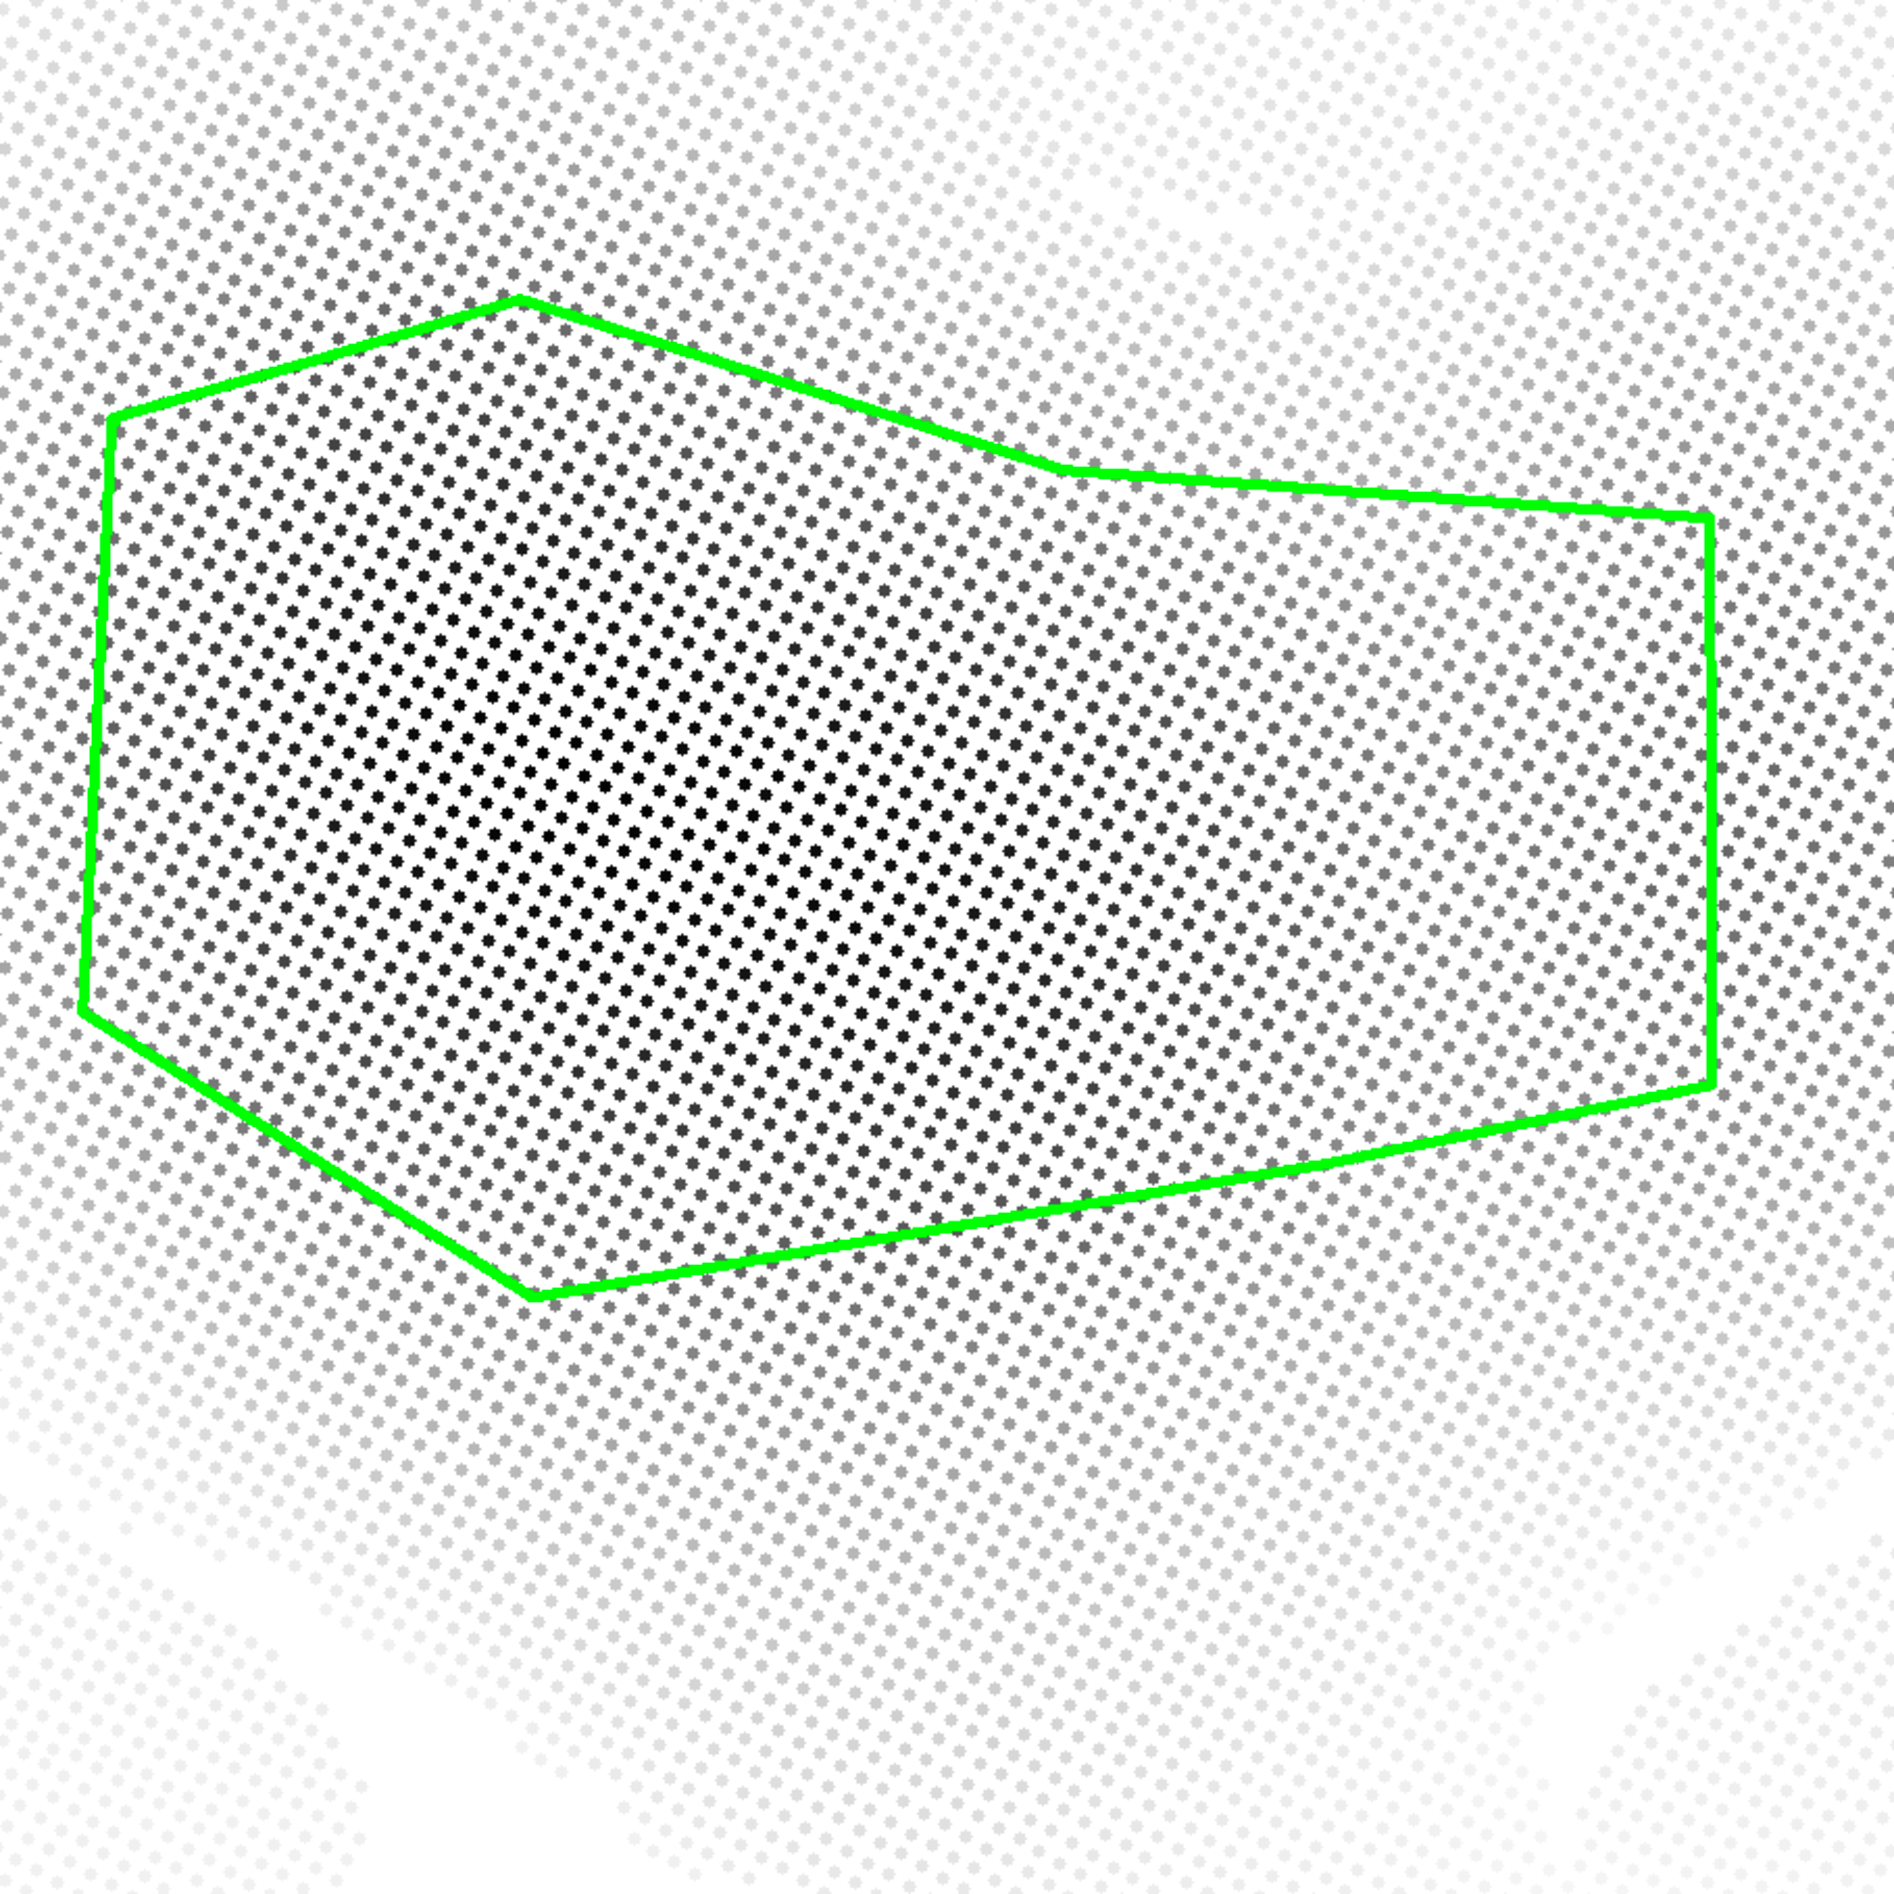
\includegraphics[width=.85\textwidth]{mask_3.pdf}
		\caption{Masked XCF Map}
		\label{fig:mask_t_3}
	\end{figure}
	
	\item Once you are happy with your selection you can save the current selection by selecting "Polygon Selection > Save Selection" from the menu appearing after another right-click as shown in \autoref{fig:mask_t_4}.

	\begin{figure}[H]
		\centering
		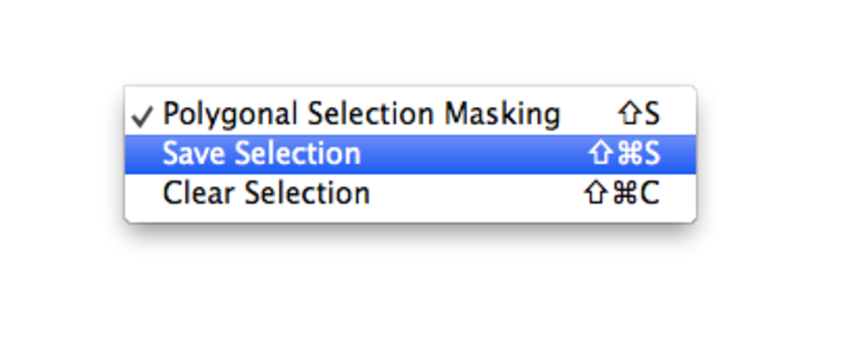
\includegraphics[width=.65\textwidth]{mask_4.pdf}
		\caption{Save the drawn polygon}
		\label{fig:mask_t_4}
	\end{figure}
	
	\item In order to apply your polygon selection you have to run the custom script \textit{Mask Crystal from Polygon}. This script will replace all the pixels outside the polygon with the average grey value inside the polygon. In the future calculation this new image will be used as input image.
	
	\item After masking the crystal from the saved polygon you have to save the current configuration by means of clicking on the save button in the header of the {\twodx}\texttt{\_image} graphical user interface. Afterwards you have to rerun the following standard scripts:
		\begin{itemize}
			\item \textit{Calculate FFT}
			\item \textit{Get SpotList for Unbend I}
			\item \textit{Unbend I}
			\item \textit{Get SpotList (complete)}
			\item \textit{Correct CTF}
			\item \textit{Generate Map}
		\end{itemize}
	
	This will generate a density map uniquely from the data points inside the selected polygon.
	
\end{enumerate}


\subsection{Synchronize Project}
\index{Synchronize Project}
\label{sec:sync_project}

{\twodx}\texttt{\_merge} allows you to synchronize your data with a different directory through the custom script \textit{Synchronize with Backup}.








